\chapter{Les Types d’Apprentissage Automatique}
\label{chap:types}

\section{Apprentissage Supervisé}
\label{sec:supervise}
L’apprentissage supervisé est un modèle qui apprend à faire des prédictions ou à générer des résultats souhaités en se basant sur une série d'exemples étiquetés, c'est-àdire des données accompagnées de la valeur à prédire. Ses principaux avantages
résident dans sa simplicité et sa facilité de mise en œuvre. Il est particulièrement utile pour prédire un nombre restreint de résultats possibles, classer des données en différentes catégories ou combiner les résultats de plusieurs algorithmes de Machine Learning.


\subsection{Classification}
Dans le domaine de l'apprentissage automatique, la classification est une technique permettant de catégoriser des données en classes prédéfinies en fonction de leurs caractéristiques. L'algorithme apprend à partir de données étiquetées, où chaque point
de données est associé à une étiquette ou une catégorie spécifique. Le modèle a ainsi pour but d'assigner une valeur discrète à une donnée d'entrée. Par exemple, déterminer si un courrier électronique est un SPAM ou non constitue un problème classique de classification.




\subsection{Régression}
La régression est une méthode d'apprentissage automatique qui permet de prédire ou estimer la valeur d'une variable dépendante en se basant sur les valeurs d'une ou plusieurs variables indépendantes. Contrairement à la classification, elle vise à prédire des valeurs continues en attribuant une plage de valeurs à une donnée d'entrée. Elle est couramment utilisée pour des tâches telles que la prédiction des ventes, l'estimation du prix des maisons, des salaires, etc.

\begin{figure}[h]
    \centering
    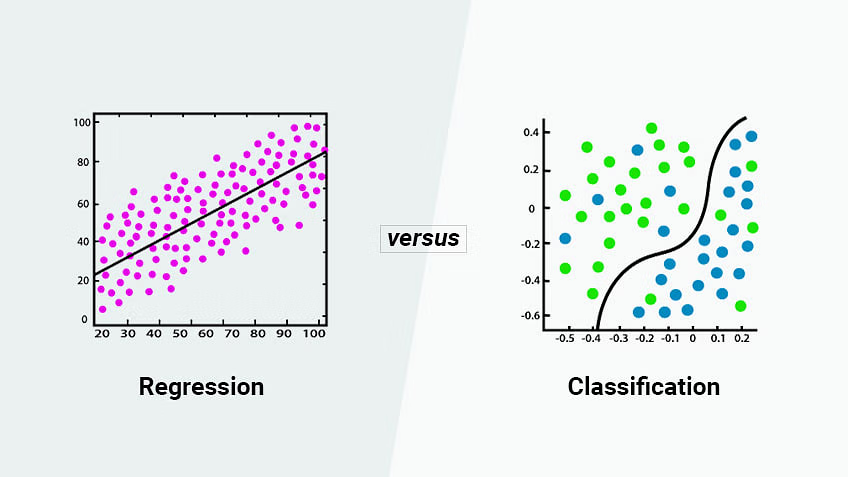
\includegraphics[width=0.7\textwidth]{Imag/Regression_vs_Classification.png}
    \caption{Régression vs Classification}
    \label{fig:mon_image}
\end{figure}

\section{Apprentissage Non-Supervisé}
\label{sec:non-supervise}
L'apprentissage non supervisé est une branche du Machine Learning qui utilise des données brutes, non étiquetées ni classées, pour entraîner les modèles. Il permet de découvrir des structures cachées dans ces données, comme la reconnaissance de motifs
ou la détection d'anomalies, ainsi que d'organiser automatiquement les données en groupes pertinents. Cette approche est avantageuse car elle ne nécessite pas d'étiquetage préalable des données, ce qui simplifie sa configuration.

\begin{figure}[h]
    \centering
    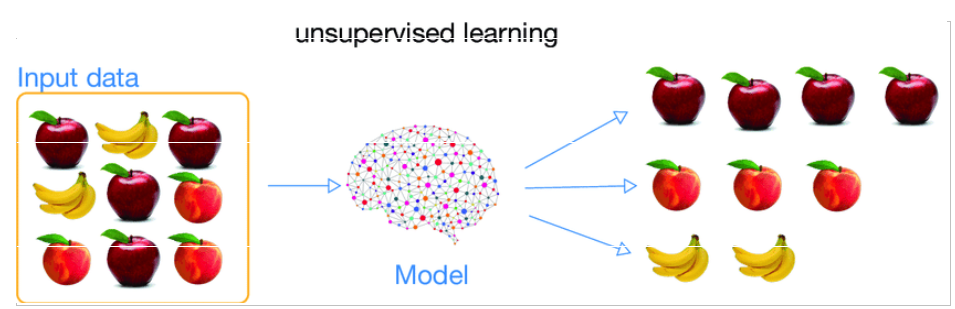
\includegraphics[width=0.7\textwidth]{rapport/Imag/2020-10-28-10_41_58-Machine-Learning-vs-Human-Decision-Making.png} 
    \caption{L'Apprentissage Non Supervisé}
    \label{fig:mon_image}
\end{figure}


\section{Apprentissage par Renforcement}
\label{sec:renforcement}
L’apprentissage par renforcement (RL) est un processus de machine learning axé sur la prise de décision autonome. Le terme « agent autonome » désigne tout système capable de prendre des décisions et de réagir à son environnement sans instructions directes de la part de l’humain. Les robots et les voitures autonomes en sont des exemples. Avec l’apprentissage par renforcement, les agents autonomes apprennent à effectuer des tâches selon la méthode essai-erreur, sans être guidés par l’humain.1 L’apprentissage par renforcement s’attaque notamment aux problèmes de prise de décision séquentielle dans un environnement incertain, et promet d’accélérer le développement de l’intelligence artificielle.

\section{Techniques de Classification Appliquees}
\label{sec:Techniques}

\begin{itemize}
    \item Regressions Logistiques: Ideale pour pr´evoir la probabilite qu’une classe specifique produise un defaut. Simple mais efficace pour des problemes
lineaires.
    \item Forets Aleatoires (Random Forest) : Constituees de multiples arbres de decision, elles offrent une robustesse et une precision accrue en reduisant le risque de surapprentissage.
    \item Support Vector Machines (SVM) : Particulierement utile pour des espaces de donnees complexes. Cherche `a maximiser la separation entre les classes.
    \item K-Nearest Neighbors (KNN) : attribue une classe à une nouvelle donnée en fonction des K points les plus proches dans l’ensemble d’entraînement. La classe majoritaire parmi ces K voisins est choisie pour prédire l’étiquette de la nouvelle donnée.

\end{itemize}

\begin{table}[h!]
\centering
\setlength{\tabcolsep}{4pt}  % Réduit l'espace entre les colonnes
\small  % Réduit légèrement la taille du texte

\begin{tabularx}{\textwidth}{|X|X|X|X|X|}
\hline
\textbf{Algorithm} & \textbf{Regression, Classification} & \textbf{Purpose} & \textbf{Method} & \textbf{Use Cases} \\
\hline
Logistic Regression & Classification & Predict binary output variable & Logistic function transforming linear relationship & Binary classification tasks \\
\hline
Random Forests & Both & Improve classification and regression accuracy & Combining multiple decision trees & Reducing overfitting, improving prediction accuracy \\
\hline
SVM & Both & Create hyperplane for classification or predict continuous values & Maximizing margin between classes or predicting continuous values & Classification and Regression tasks \\
\hline
KNN & Both & Predict class or value based on k closest neighbors & Finding k closest neighbors and predicting based on majority or average & Classification and Regression tasks, sensitive to noisy data \\
\hline
\end{tabularx}
\caption{Machine Learning Algorithms and Their Applications}
\label{tab:ml_algorithms}
\end{table}     % Tableau comparatif